\documentclass[a4paper,11pt]{report}
\usepackage{geometry}
\usepackage{graphicx}
\geometry{left=1.5cm,right=1.5cm,top=1.5cm,bottom=1.5cm} 
\renewcommand{\baselinestretch}{1}
\begin{document}
\title{%
	7CCSMPRJ Individual Project 18-19\\
	Final Report \\
	\vspace{1mm}
	\LARGE Human interaction with voice-assistant agents}

\author{%
	\LARGE Thomas James Robinson\\
	1880679\\
	thomas.robinson@kcl.ac.uk\\
	\vspace{5mm}\\
	Supervisor: Petr Slovak
	}

\date{August 2019}

\maketitle

\chapter*{Abstract}%
\addcontentsline{toc}{chapter}{\numberline{}Abstract}%
This paper will outline the design and implementation methods conducted to create a device capable of recording quality conversations that can be used in a therapy session for parents who have sought out an intervention to help them raise a child. This paper will examine the importance of parent-child interactions and study the links between these interactions and the development of mental health issues in young people. There will be discussion on what information is important for a therapist to hear and in what situations are there likely to be poor parental techniques. It will also scrutinize the current techniques used to detect conflicts and the current technological solutions available to aid in the prevention of mental health issues within a family setting. \\

The software created will make use of antecedent and ensuing recording techniques around a pre-defined point in conversation which will activate the device as this is where it thinks a conflict is taking place. The report will also outline the steps needed to export the software to a Raspberry Pi device and how important this is to the potential success of this project. There will be a short discussion about the use of cloud storage as this device will upload files to a shared online space.\\

This papers contribution to the field of Human Computer Interface is the first comparisons between Dyadic Parent-Child Interaction Coding Scheme and Social Signal Processing, an emerging technological field used to track humans’ actions and underlying intentions. Utilizing this technology could bring a whole new level of quality information to the therapy sessions that can help in the detection of poor parenting and prevent the early development of issues in children.\\

\pagenumbering{roman}
\tableofcontents
\newpage
\pagenumbering{arabic}

\chapter{Introduction}
For the duration of this academic year I have been researching how human interaction with voice assistants can be used to provide mental health interventions. I specifically have been researching the detection of the audio and how to activate notifications for the user at certain points within the conversation. I have also been researching if and how this can be implemented into voice assistants already embedded in the home. The core build for my project will be to create a ‘path’ for audio input to travel down in which I will provide functionality at ‘anchor points’, points at which I feel an intervention is needed, alerting the user that the system has been activated. This will in turn provide feedback for parents in the prevention of mental health problems in young people. One specific anchor that I will be looking at implementing is shouting within a conversation, this is because if a conversation has reached the point where shouting or slamming of doors occurs it is likely this conversation includes a conflict which would be useful for a therapist to analyse. The prevention of mental health issues will come in the form of therapist sessions, in which the therapist will be able to dissect the conversations where the conflict occurred. There is also potential for the professional to leave comments on recordings, which can give the participants something to work on in between sessions. \\

When my software has detected increased volume of sound, it will store a certain amount of audio leading up to the anchor point and a some after, this could either be a certain amount of time or until the shouting has stopped. This audio could then be sent to the users for review or sent to a third party to be analysed e.g. a therapist. The system will also aim to detect if there is silence after the shouting has taken place as an indicator as to whether the conflict was resolved or if one participant has shouted and immediately left the conversation. This project is needed because there is a limit on the quality of conversation that can be gathered from in-lab experiments, as it is more likely that the patients will change their dementor knowing they are taking part in an experiment. Placing a device into the home will increase the chances of hearing more natural conversations and therefore increase the quality of conversations available to therapists. \\

Voice assistants are a relatively new technology and this means that there has been little research into how effective they can be as a tool for assisting with health-related issues, there are multiple \textit{skills}\footnote{Skills are the applications equivalent for Amazon’s Echo series. They are activated by audio commands.} that allow Amazon’s Echo to become a personal trainer ( (Amazon, 2017) (Amazon, 2017) (Pargee, 2015)). However, there has been little research directly involved with supporting with mental health (aside from meditation skills), which is the main focus of my report, hence motivation for this project is hoping to help solve a real-world problem with an emerging technology. Mental health problems have a large effect on everyone involved with the patient as well as having a profound effect on health services (Simo, Bamvita, Caron, \& Fleury, 2018), with the UK committed to grow funding by at least £2.3bn a year for mental services (NHS England, 2019), it is clear to see that this is an important focus even for current governments. This project will focus more on the prevention of mental health problems developing for young people as the benefits for prevention over treatment are clear to see for both patient and governments (National Acadamies Press (US), 2009). Being able to detect conflicts a young child hears will allow professionals to apply parenting coding schemes, such as the\textit{ Dyadic Parent-Child Interaction Coding System}. These systems outline parental techniques that therapists have highlighted as specific actions that either have a positive or negative affect on the child (most of which occur within a conflict), hence the reasoning to detect conflicts. \\
 
Within this project I will also be examining related systems currently on the market to understand the differences between them and to find the most effective methodologies for prevention. Most of the current techniques have been found to influence participant’s actions, whether that be a clinical trial, within a staged environment or within a home environment with a more observational method. Therein lies the importance of this project, allowing conversations to be recorded that are in the home environment without having the people conducting the experiment in the home observing them. To achieve this, I have created a device that captures conversations in a home environment that is less likely to influence participants actions. This device will then upload the conversations that contain conflicts to a shared file space, in which comments can be made on specific aspects of the recording by a therapist which will be used to help a family to better resolve conflicts and implement the good techniques identified in certain parental coding schemes.\\

 I have also been researching various coding techniques\footnote{Coding = Categorising of data} , including DPICS, for parenting observation which will be discussed at length later in this report. This project will use some external libraries for the algorithms for audio detection and uploading of files to Dropbox. I have found that most of the successful and robust scripts for this are written in Python (e.g. \textit{PyAudio}), so for this reason, the software will be written in Python. Success in this project can be gauged by whether the device can detect conflicts arising within the home environment at a better rate and quality than the devices and techniques currently being used.\\


\chapter{Literature Review}
Within this section I will be reviewing current literature related to the use of voice assistants in assisting prevention of mental health issues. As this is a relatively new area of research I will also be referencing uses of voice assistants for other uses outside of the ‘\textit{normal}’ day-to-day functionality, as well as the use of audio \& screen analysis. The focus of this reviewing will be on how they handle the audio and create the anchor points at which to provide feedback to the users. There will also be a review of the importance of placing an emphasis on the prevention of mental health issues over the treatment of these issues as this is what my system will aim to assist with. In addition, there will be a mention of the acceptance of home hubs recording audio without direct authorisation of the user with an ‘activation word’ being used. I will be analysing current coding techniques used to review parental methods during parent-child interactions and how these could be detected with audio analysis. I will be reviewing the algorithms in which audio patterns are currently detected. 

\section{General Background}
I am going to start by analysing the background and need for this system. Approximately 1 in 4 people in the UK will experience a mental health problem each year (NHS, 2007) and within England, 1 in 6 people report experiencing common mental health problems, \textit{anxiety and depression}, in any given week (NHS, 2014). With so many people being affected by mental health issues it has become clear to governments that this is an issue that needs be addressed and as mentioned above there the UK government has committed to increasing spending in this area for the long term. \\

Looking specifically at young people, mental health problems affect about 1 in 10 children but 70\% of children and young people experiencing these problems don’t have appropriate intervention (Mental Health Foundation, 2019), this is what this project is aiming to help. Research has led us to believe that prevention of mental health issues is a more effective and beneficial way of handling this world-wide problem than trying to treat sufferers ( (World Health Organisiation, 2003) (Zubrick, Silburn, Burton, \& Blair, 2000) (Andrews \& Wilkinson, 2002)). Prevention has been identified as the most effective way to combat mental health issues in older generations, with late life depression being commonly associated with high rate of mortality (Charney \textit{et al}, 2003). The Institute of Medicine’s Report on Prevention of Mental Disorders identifies terminology to describe preventitive interventions (Figure 1) (Mrazek \& Haggerty, 1994).\\

This project, given the appropriate approval and collaboration, could be imbedded into homes with ‘always-on’ technology to create a system that would be an effective means of notifying users and possibly become an intervening agent in situations where young people’s mental health could be at risk, which would be at the ‘Primary Prevention’ stage from Figure 1. \\

\begin{center}
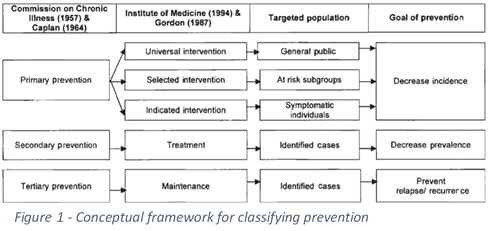
\includegraphics{Framework.PNG}
\end{center}

As with any new technology, acceptance of this into our lives comes under immense scrutiny (Kääriä, 2017). This is especially the case when said technology is embedded directly in the home, where the most intimate family moments take place. Systems like \textit{Amazon Echo, Google Home and Apple HomePod} are not immune from this scrutiny, with tabloids and articles manipulating people into thinking negatively about voice assistants (Baker, 2019). This is relevant to this project as this system will aim to listen to conversations without direct authorisation from the user. With audio being recorded for a time before and after a certain volume being recorded it may be hard to gain acceptance for a system like this in the public domain.\\

\section{Current Literature \& Related Works}
This section will review works related to the development of voice assistance and ‘always on systems’ especially within the context of preventing mental health issues. It will also consider other activities outside its regular use, some examples of regular use include; asking the device to play a song, to set a timer and asking for weather updates. Regular use is further defined in ‘Voice Interfaces in Everyday Life’ (Porcheron, Fischer, Reeves, \& Sharples, 2018) which analyses the way which families use such devices in their everyday social interactions by deploying an Amazon Echo device into homes for a month, along with a purpose-built Conditional Voice Recorder (CVD). This CVD captures audio of the last minute in a temporary buffer. When an activation word is used (“Alexa" for Amazon Echo), it will save a prior minute of recording and another further minute past this point. They then focused on the way the participants ‘requested’ certain actions and were interested in how participants organised their actions with and around the Echo. This paper also addresses the use of the Echo with different members of the family, with two of the participant families involving 2 adults and 2 children, with one family struggling with Amazons ‘equal access’ conditions as the children direct \textit{Alexa} to do something halfway through a command from a parent. This is something which could transpire into a disagreement between the two parties, the system would then have the preluding conversations to this disagreement which could then be sent to the user or to a third party for analysis. \\

This is one example of where this project potentially overlaps with mine. The CVD, with its ability to maintain the last minute of audio recording before activation is something which I am considering implementing into my system as this will allow users to see what led up to the shouting (my activation point). The overlapping continues with the next minute being recorded and the subsequent minutes if the activation point is met again. This allows for a continuous stream of a conversation to be analysed, something which will be vital in analysing a full conversation thread. Another overlapping goal is to break down interactions that occur near the system as both systems are analysing the way which humans communicate.\\

Another work that has a similar outline to mine is ‘Anchored Audio Sampling’ (AAS) (Hiniker, Froehlich, Zhang, \& Beneteau, 2019). This report also works with antecedent and ensuing audio recording (Figure 2), but is analysing the benefits and drawbacks of AAS. It does this by implementing AAS into 3 case studies. First, \textit{Pre-schoolers’ Video Transitions}, where they recorded the audio surrounding a video on YouTube ending and the next one starting to see if they could increase efficiency at this point. Next, \textit{a tablet application to train executive function}, where they looking to see if the application was training executive functions which have proven to be a strong predictor of a number of outcome measures later in life. Finally, a case study of \textit{Families use of Amazon Echo Dot}, which was similar to the above paper where they recorded a minute before and after the word “Alexa” was used. All three case studies involved children. \\

One of the main benefits they found with AAS was that antecedent recording gave them a further insight into why things occurred. This is shown from the third case study where they were able to decipher why certain requests were made, the example in the paper is when a child requests a number between 3 and 5. On analysis it became clear they were deciding what time to leave for an event, if the system knew that this was the full request the Echo Dot may have replied with a more accurate answer. Some drawbacks included the participants being aware of the recordings and altering their behaviour as they knew they were being observed, this was evident in study 3. They also found that, although they still received a large amount of useful data from audio, they were unable to create a complete picture of the usage without a visual data.\\

\begin{center}
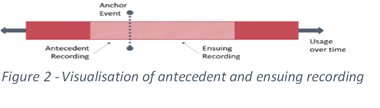
\includegraphics{Recording.PNG}
\end{center}

The case studies in this report have many similar techniques for achieving its goals as my project; the antecedent and ensuing audio recording is the main method of gathering data from the participants. The main difference in my project from the case studies is the anchor point that I will be using. My system will be activated from an increased volume from one of the participants. This paper has outlined some of the most important benefits as to why this type of recording is useful for capturing humans’ part of HCI. What is especially useful is that all of these case studies were involving children, which are the focus of my studies. This paper has also outlined some of the important factors to consider in design of the system as well as factors to consider when analysing any results from the deployment of a system of this kind; participant’s awareness of recording and not being able to see the whole picture. What is concerning is that the case where the participants changed their actions was the study with the Echo Dot, as this was the study that is most similar to mine. \textit{Anchored Audio Sampling} also reported on how difficult they found it to find families that were willing to participate in the test and how that they feared the results they acquired were only reflective of a certain type of family that would allow participation in studies such as this, something that must be considered for this project also.\\

A project that is related to both HCI / HCC\footnote{HCI – Human Computer Interaction, HCC – Human Centred Computing}   and participants mental health is \textit{Predicting Symptom Trajectories of Schizophrenia using Mobile Sensing} (Wang, \textit{et al.}, 2017); for this project they created a system named \textit{CrossCheck}. CrossCheck is a system that utilises mobile phone sensors to collect data in aid of monitoring and identifying subjective and objective indicators of psychotic relapse, especially for patients with schizophrenia. With this project they had clinicians administer a 7-item Brief Psychiatric Rating Scale (BPRS) throughout the trail to measure psychiatric symptoms associated with schizophrenia\footnote{These include tests for grandiosity, suspiciousness, hallucinations, unusual thought content, conceptual disorganization, blunted affect, and mannerisms and posturing}. The need for the system comes as clinicians cannot track deterioration of health between visits, meaning they are likely to miss the optimal time to intervene and treat patients. The system will predict patient’s weekly 7-item DPRS total scores using passive sensing and self-reported ecological momentary assessment (EMA) responses from smartphones. The clinician is still responsible for interpreting the weekly results from the tests. The app continuously infers and records participant’s physical activities, sleep and sociability, it also collects; audio amplitude, accelerometer readings, light sensor readings, location coordinates, application usages and call logs. The app uses a built in MobileEMA component to administer self-reported EMAs.\\

\begin{center}
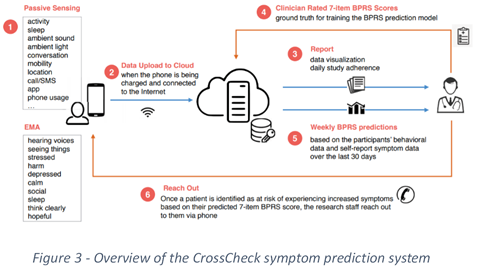
\includegraphics{CrossCheck.PNG}
\end{center}

There are many similarities between this project and mine. The first similarity is that there is a passive sensing occurring in both projects. Where this system will passively sense via multiple outlets to collect data, my system will be passively sensing via a microphone. In both cases there is opportunity to send the data away to be analysed or sent directly to the participant, although this is not implemented in CrossCheck. In both pieces of work there is a focus on preventing a mental health issue arising by utilising an emerging technology and a technology that is supposed to capture a normal day for the patient. This is further evidence that trials that occur in a natural environment and away from a lab provide a better insight into patient’s health. Something that this system does well is the communication and regular update of goals from the clinician with the patient to stay on top of the potential issues. This gives everyone involved a greater understanding of how the patient is progressing, allowing for more informed interventions to take place if they are needed. \\

The main differences between the projects are that my project is looking more at the interactions between two participants, e.g. how the parents interact with their children or other adults. This is something that this system has explicitly said it would not record, mainly due to privacy concerns. My project would not encounter this problem as often as the focus is on the parental relationships. Although \textit{Predicting Symptom Trajectories of Schizophrenia} using Mobile Sensing is aiming to prevent a relapse of a psychotic episode, my project is looking to intervene before any kind of issue occurs so would be placed earlier in the prevention timeline. My system could potentially be used to prevent people from needing CrossCheck in the future.\\

Summary:\\
From reading the literature in this section, there are still some gaps in the research area which I have identified here. In ‘Voice Interfaces in Everyday Life’, among other papers, the system designed wanted to record the human-to-system communications and there is no analysis for human-to-human interactions which make up parent-child interactions. Another common theme in these papers is the activation of the system. Most of the work reviewed the system is activated using a single word, my system is looking for a raised voice as the ‘anchor’ point instead of the word “Alexa”. This is a more appropriate anchor point for the types of conversations that I wish to be analysing as it would unnatural for someone say “Alexa” during the middle of an argument. If the system can be activated by something that is naturally likely to occur in the conversation it is more likely to pick up important sections of conversations. Of the papers I read regarding the association between HCI and mental health, there was more of a focus on those already diagnosed with the issue and little research done into projects that aim to aid the pre-treatment phase. This project is focused on the pre-treatment\\

From the research I conducted there is an agreement that accessing the antecedent and ensuing recording will give those analysing the data more context, this can be seen in the paper by Hinker et al. Across all the studies outlined here (apart from Voice interfaces in Everyday Life) it seems as if there is a shift towards using mobile phones as the medium to collect information from. This makes sense as these devices are nearly always on a person throughout the day, the only concern I have with this is having muffled conversations as phones are often placed in pockets, blocking clear recording.\\

\section{Review of Current Techniques}
\subsection{Psychological Techniques}
This section reviews the current psychological techniques used for categorizing parent-child interactions into good or bad interactions. One of the most used coding manuals for parent-child interactions is DPICS (\textit{Dyadic Parent-Child Interaction Coding System}) (Eyberg, 2000), DPICS is a detailed list of various key behaviours that can be observed in a parent-child interaction alongside multiple examples of these moments observed in experiments. DPICS is used to assess the ways parents interact with children, provide a guide to treatment and track behavioural change in therapy. Its main goals are to serve as a baseline \textit{pre-treatment} assessment of family interactions, provide measure of progress during therapy and to be a behavioural observation measure of treatment outcomes. There has been an extensive research in recent years to review the way in which we observe parent-child interactions, with a shift away from clinical trials and trying to place more emphasis of observing families in their homes to get a better view of what real life is like for these families. Table 1 below is taken from \textit{Observation Measures of Parent-Child Interaction: An Introductory Review} (Aspland \& Gardner, 2003), which outlines 28 of the parental behaviours that have been outlined in the latest version of the DPICS manual as areas that should be addressed in therapy. Here it is also compared other coding schemes, namely; \textit{The Behaviour Coding Scheme} (BCS), developed by Forehand and McMahon and \textit{Relationship Process Code} (RPC) (Dishion, Rivera, Jones, Verberkmoes, \& Patras, 2002).\\

\begin{center}
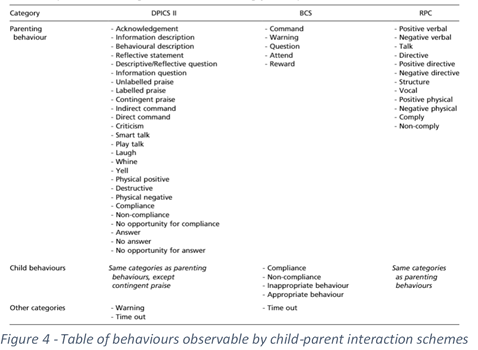
\includegraphics{ParentalCodingSystems.PNG}
\end{center}

As you can see from the table, DPICS is the most comprehensive scheme to detail various interactions between parents and children. DPICS is a good comparison of a human-to-human coding scheme that could be computerised into an emerging technology such as voice assistants for my project as it has many of the same goals; one of these is that it aims to be placed at the same point of the prevention timeline as my project (\textit{pre-treatment}). Although my project is focused on achieving a single activation point (when a certain volume is reached), this will hopefully capture a large amount of the 28 techniques in DPICS as it records a conflict rather than looking for a specific technique. It will be possible to track progress as more and more conversations are recorded as comparisons can be drawn across files.   \\	

\subsection{Technological Techniques}
In this sub section I will be reviewing voice detection and activation systems in an attempt to find the most effective ways to detect sound for my system, starting this research by testing the speech recognition package from \textit{pypi.org} (Zhang, 2016). This system is essentially a library for performing speech recognition that takes support from multiple APIs/engines including; \textit{Google Speech Recognition, Microsoft Bing Voice Recognition} etc. This system also requires PyAudio to be installed on the terminal, PyAudio provides Python bindings for \textit{PortAudio} which itself is a library that provides simple API for recording. When you first open this package, you must select which API you wish to use to parse the audio you are going to input to the system, I selected Google Web Speech API for testing.\\

There are many things this project highlights that could are related to my work, the ability to use both a pre-recorded audio source and also live recording from a microphone (allowing for real-time analysis of a conversation) is one of those things. One of the most interesting aspects of this system was its ability to have automatically varying figure for depleting background noise. This is a useful tool to have as the goal for my system is to be placed in the home, an environment that is likely to have varying amounts of background noise. This skill allows a system to focus on the main topic of the recording. The main thing this system does well is track what is being said by the participants. Although this isn’t specifically needed for the detection of raised voices, having this already in the system would make it easier to create other anchors surrounding certain phrases or words. This is where the main differences lie between my project and this one, this system is specifically aimed at reproducing the audio as text and has no capabilities to detect changes in volume or create notifications at any point. As mentioned, this system has many good aspects that can be transferred into a volume detection system but it has not been created with any other purposes in mind.\\

Another project that has a closer goal to mine is \textit{BarkTracker} (Lindsey (\textit{f4ngy}), 2014). This project is designed to send an e-mail notification to someone when their dog is barking and the system is running. This works by setting an ambient decibel level and if this is exceeded then a notification is sent to the user. BarkTracker also has a timer of 15 minutes that starts after it hears an initial bark, during this time there cannot be another notification sent to the user about the noise being heard. When the email is sent to the user it includes just the basic information of the time that the noise occurred.\\

In its basic form this has a major similarity to my project, with both monitoring sound in the home and having decibel (db) level as an anchor point where a notification is sent to the user. This is where the similarities end, with the main differences being what is contained within the message. Another weak part of this project is that the ambient noise level is not variable. Although it can be changed within the code, this level would not be accessible to the user on an executable version, meaning if the system was moved into another room or if there was another foreign source of noise that wasn’t there on set up the system will be recording more often at incorrect points as the db level will be constantly raised. The timer between sending notifications is also something that would not benefit my system as even if there were multiple arguments within the time period, they are still all useful to the users.\\

The last system I will be reviewing is \textit{Decibel X} (SkyPaw Co. Ltd, 2017). This application is available on Apple app store and Google Play store. Decibel X is a detailed decibel level meter that that gives the user a comprehensive overview of the sound that can be heard from the device and gives a recommendation as to the similar levels of sound. This application gives the user the option between a live FFT or bar graph which are useful for sound analysis; it also gives the option to change between weighting filters (dBA, dBB, dBC \& dBZ). A-weighting is the universally accepted weighting that is used for all standards that correspond to human hearing. Decibel X also allows for the audio to be recorded and saved alongside the raw information that is shown on the UI, this information can then be saved into the cloud or into the local device. The UI also displays; current, average and max decibel levels reached.\\

Comparing this to my system, there are many differences between the aims and objectives. Decibel X aims to give a detailed breakdown of the sound heard in the environment, something that I am not particularly concerned with giving. There are some things that could be useful for users of my application with the ability to retrieve a summary which includes; duration, average and max levels of audio heard. The main thing that is similar with this system is that it analyses sound and can track decibel levels. This is the basis of my application and this system is able to do so with great accuracy which is important when working with a sensitive subject matter like that in my project.\\

Summary:\\
From researching the current psychological techniques, it seems as if the common theme among the paper is a focus on trying to move away from clinical trials. The DPICS manual was initially used with clinical trials and has since moved into observing home interactions. My project aims to take this one step further and observe the home without having to place an actual person in the home. Another area that seems to be lacking is the recording of the right information. With many of the psychological techniques having to analyse lots of data it could take a long time to find appropriate conversations.\\

From reviewing the technical techniques currently used to record conversations or noises it is clear there is a lack of research into how this can be used to aid the detection of mental health issues. Although there are many things these systems already posses that would make them useful in this field (use of PyAudio). This can be seen with the BarkTracker application, that contains many useful ideas that could be used to help in this area, but instead is focused on tracking barking from a dog. Similarly to the above section, there is an affection towards detecting specific words with many systems that I found, this is highlighted in speech recognition package and even though this skill would be important for implementing a system that was focused on some of the specific parenting techniques in DPICS, it is not relevant for my project. Following on from this it seems as if there is little to no commercial applications available that detect conflicts.\\ 

From the applications named above it seems as if there is not an application made that carries the appropriate data that would be required for a clinician to analyse conversations in the home. From the BarkerTracker the information included is simply not enough data as this just a notification that there was an instance of reaching a high decibel level. For Decibel X, this application contains too much detail which is not required and would just end up wasting space on drives / shared spaces. A common theme for these applications, and many applications generally, is the requirement for them to be connected to the internet to achieve their goals. Although this feature may become part of my application, having a device that can still reach its goals independently of connection to the internet is something that is missing from this area.


\section{Social Signal Processing}
This section will review Social Signal Processing, SSP is a relatively new way for machines to analyse human emotion, which accounts for a large portion of our social intelligence. Some have argued that social intelligence has become one of the key features a person can have to lead to success in life (Goleman, 2006). If this is the case, then it could be argued that those who suffer from social disabilities are inherently less likely to succeed in life If this in turn is the case, then these disabilities must be diagnosed and treated as early as possible as to reduce the impact they could potentially have on a child’s life. As I mentioned at the start of this section, social signal processing is still a relatively new field (2009) but there is evidence to suggest current techniques and algorithms can identify the ‘Ekman Big Six’ emotions of: Anger, Disgust, Fear, Happiness, Sadness and Surprise (Figure 5). It has also been known to identify everyday emotions of interest, pleasure, relief and stress; social emotions of embarrassment, guilt, pride and shame (Scherer, Schüller, \& Elkins, 2017); and some continuous models show that it can interpret arousal, valence dominance, novelty or intensity. \\

\begin{center}
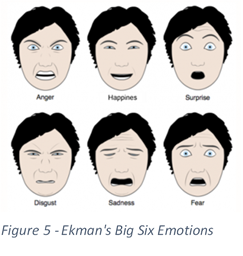
\includegraphics{Ekmans.PNG}
\end{center}

For a lot of these emotions to be observed by a system they require the system to analyse signals being output by the subject from multiple domains (facial expressions, actions taken by parties involved and other physical elements). As my project will be based on the observation of sound I will be discounting these techniques in this study. Some of the most popular techniques that have been used to observe the remaining emotions through sound include: Time Domain (\textit{Duration of utterance, voiced parts and silent periods + speech rate}), Frequency Domain (\textit{How often one is talking over an interaction}), Amplitude Domain (\textit{Intensity of utterance or increasing intensity over interaction}) and Spectral Domain (\textit{Voice quality measures}). These techniques are yet to be fully explored in the research domain, especially in the detection of potentially harmful interaction between a parent and a child, although they have been used for some novelty applications. Examples of this include ‘Lie Detector Truth Test’\footnote{Available to see on Apple App Store: https://apps.apple.com/gb/app/lie-detector-truth-test/id1113503715} which, as the name suggests, aims to detect of someone is lying by analysing voice clips. There are also apps that will aim to detect stress and others aiming to detect “Love” (\textit{Affection}). \\
 
Another interesting area SSP has explored is that of Automatic Role Recognition (Vinciarelli, Social Signal Processing for Automatic Role Recognition, 2017). This is particularly interesting for studies that include parent-child interactions as there are certain expectations for both roles within an interaction, with an emphasis on how the parent reacts to certain situations for my project. Previous work has been done in identifying more detailed roles including giver, seeker, recorder, neutral and orienteer. Within the same work they have been able to identify socioemotional roles like gate-keeper, supporter, protagonist and attacker, some of these socioemotional roles are likely to be observed during a parent-child interaction (gate keeper, supporter) and the others are likely to be observed during an argument. Being able to identify when someone is or isn’t playing these roles could be important information when analysing an interaction which has been tagged by a system for containing something adverse between a parent and a child.\\

According to Cheng \& Cristani vocal behaviour can also be used in surveillance as there are many social cues that can be picked up by the way that one expresses an utterance. There are five main components that can analysed through voice (Cheng \& Cristani, 2017): Prosody (\textit{For competence}), Linguistic vocalization (\textit{highlighting hesitation}), Non-linguistic vocalization (\textit{proof of close bonds}), Silence (\textit{hesitation}) and Turn-taking patterns (\textit{can more accurately model conflict interactions}). Schegloff (Schegloff, 2000) proposes that during arguments overlapping speech becomes both longer and more frequent as the participants struggle to ‘hold the floor’ and stop the other from speaking. This is something that could be explored within my project also.\\

Conflicts are an area that is still to be fully explored within SSP (Vinciarelli, 2017). This is mainly due to the recordings made public tend to be agreeable situations, so the conversations heard do not contain conflicts. As conflicts deals with such personal information there is even less desire to share this information with researchers. On top of this fact is that there has been limited research into how conflicts start and develop within social psychology as well. This will likely soon change as conflicts are shown to be the interactions which one expresses their emotions clearly as they struggle to persuade the other party to adjust their views to align with their own, hence why I have decided to make conflicts the main focus of my study. \\

As SSP can pick up on these subconscious cues within a conversation and given the correct placement within a home, it is in the unique position of being able to aid the detection of developmental disorders with emerging technology. This has been explored with attempting to detect signs of a child being on the autism spectrum, as some type of autism can affect one’s desire and ability to speak. This paragraph will look beyond just sound analysis to assist with detection. One thing that may become a key sign in detection of these early developing disorders is synchrony (or lack thereof). In the dictionary synchrony is defined as “simultaneous action, development, or occurrence”. In terms of development for young people interpersonal synchrony could mean the production of communicative signals, including speech. Chetouani et al have found evidence for robotics playing different roles during interactions with children to varying success, including: Robots used to elicit behaviour, Robots used to model teach or practice skills \& Robots used to provide feedback and encouragement (Chetouani, Boucenna, Chaby, Plaza, \& Cohen, 2017). Even though this is still a new area for SSP to explore there is already been great progress made and a sign that technology can give us further insight into the mental health of young people, something that I hope this project can be a part of.\\

One thing that I have found across multiple sources is that early detection and treatment of mental health issues is important for these issues to have as little effect on the patient as possible (Skills For Care, 2018) (Trueman, 2015). Also outlined in ‘SSP and Socially Assistive Robotics in Developmental Disorders’ is a further 9 points that they have found to be effective tools for treatment through various literature pieces, these can be found in Appendix 1.\\

Even though SSP has covered a wide range of concerns and addresses many issues there are this some things that are not considered and accounted for in current research. One of the main problems is the cultural differences that could be at play within each household/interaction. Every household will have a different order and way of flowing so it would be improbable for there to be a blanket standard that we would want implemented across all participants. This is also something which would be counter productive for society as diversity and different personalities are what make up a community, which can be just as important to young people’s mental health as home relationships. Another issue that has been raised within SSP research is that of self-presentation. As most studies have been based on recordings of clinical trials there is a possibility that the participants were not being honest about the way they would have interacted as they knew they were the subject of an experiment, these issues are similar to those discussed for DPICs above.\\

A final white spot that has been raised is the problem of ‘gating’, which is the issue of recording the right segments of data. There is no perfect formula that has been found that will only capture every altercation with no missed arguments or conversations that are not of interest. This is an area that can be improved as the understanding of SSP grows, with more definite cues outlined the technology will be able to pick up these altercations and be more certain that they are of interest to the users. Another way this can develop is through machine learning. If the programme is continually told an interaction has been incorrectly flagged and can adjust to the information without too much interaction with a developer, then more accurate results are likely to forthcoming as the machine analyses more conversations.\\

\chapter{Design}
Within this section I will first be outlining the specific aims that I have for this project as well as the objectives I will hope to fulfil when achieving these aims. I will then be discussing the various design decisions I made en-route to creating a suitable system for detecting conversations of interest with respect to the information learnt in the above sections. I will then go on to highlight how I implemented such design decisions. After that, I will be analysing the technical aspect of the project and provide an evaluation of how effective my system is and how well executed it has been.

\section{Aims \& Objectives}
The overall goal of my project is to help families and therapists better understand a subject’s home dynamic so that a therapist (or other professional) can pick up on certain parental techniques that may cause young people to suffer from mental health complications. I aim to help in this area by supplying more useful and important information for analysis as there should be a more natural feel to the conversations occurring in the home. To achieve this aim I set out to create a device that can be placed in the house, or onto a person, or into an area that will detect conversations between a parent and a child or parent-parent interaction. To create this device and its functionality I had several objectives which I set out to achieve:
\begin{enumerate}
\item Information gathered must be useful for those analysing the conversations.
\item Must correctly identify when a specific type of conversation is occurring.
\item Anchor points be unique enough, so that those dissecting information are not overloaded with data.
\item Device must be in range of ‘good’ quality conversations. 
\item Be placed in the home and be accepted as ‘part of the furniture’ and not be too intrusive on the home dynamic, so the conversations recorded reflect the real atmosphere in the house.
\item Must consider data protections laws.
\end{enumerate}
To achieve requirement 1, it will be key to decide on anchor points which to focus the recordings around, these will be the points that the device has detected there may be something wrong in conversation, much research must be done in this area before settling on a point. This must also contain ensuing conversation as to analyse the resolution of the conflict. For requirement 2 it will important to execute requirement 1 properly. 3 will depend on the research conducted for requirement 1. Requirements 4 \& 5 will depend on the hardware solution chosen, some potential solutions include software for; Phones, Voice Assistance, Stand Alone Device. Finally, for requirement 6 we must consider where information should be stored, so that it is available for professionals and subjects to have equal access to information.\\

\subsection{Objectives Compared to Literature}
When I set out these objectives, I was unsure on the anchor points but having conducted my research and completed my literature review I decided that to meet these objectives and aims I will detect shouting as the focus of my recordings. To come to this decision, I focused on what I thought Procheron et al did well in ‘Voice Interfaces in Everyday Life’, as this study is concerned with the recording of conversations that occur in the home environment and makes use of antecedent and ensuing recording to analyse a whole stream of conversation. They also managed to achieve good results from an external device placed in the home, which may be what my software is exported to, showing that there is a possibility of getting good quality conversations with a foreign object in the house (requirements 4 \& 5). The decision to cover conflicts in general came from reviewing the DPICS manual, I had to decide what type of conversation I thought would produce the most of these techniques. Conflicts as a type of conversation are likely to produce many of these techniques as it is often the case that emotions are heightened at a time like this and one is more likely to reveal their true feelings towards the other party, which would be useful information for a clinician (requirement 1). \\
 
The decision to use shouting as the anchor points came as there is many applications that are focused on the words used within a conversation, outlined above. However, after reviewing the current techniques this kind of anchor would be nearly impossible to implement effectively across many different applications of the system. This is due to the varying linguistic signatures that are associated to a specific country, region, or even family. Some families may use words that others don’t and accents would have to be taken into account, implementing this kind of system would require a test to ensure the family specific words can be picked up. Having something that is recognised as a clear sign conflict is taking place was important for this project (requirement 2). Shouting is also a unique marker and it is rarer that this could be misinterpreted compared to single words for anchor points (requirement 3).

\section{Design Decisions / Methodology}
As stated in the section above, the goal of my project was to create a listening device that can detect shouting in a conversation and record the dialog that may be important to a therapist so that this can then be dissected in a session with the parents. Here I will outline the various steps I went through to create the software including; creating an audio channel, saving the file locally, activating when the shouting has occurred, continue recording if more voices are heard, recording the conversation that occurs before the shouting is detected, exporting to Raspberry Pi and uploading the file to a shared online space. As you can see from the Project Plan at the bottom of this report, the project did not always run as planned as ideas and aims changed. This was as expected as I wanted my methodology to be agile and my project plan reflects.

\subsection{Creating Audio Channel \& Saving}
The first decision that had to be made when creating the application was which language to use to write the code in. After some research it became clear that the package Pyaudio was the most effective for recording conversations. This package is created in Python so this is the language that I used to create the rest of the application, building on the capabilities of Pyaudio to provide bindings to port audio. Python was also a clear choice for this project because of its ability to be created on multiple platforms with ease, this is also a benefit of Pyaudio as it is also it designed to work across many platforms without having to change too much of the code.\\
 
The next step was to record a conversation and then save the file locally. These are part of the core functionality of the application, so it was important that when I was able to detect sound the ability to store the audio that was heard from the microphone was to follow on from this. These two form the basis for which the rest of the project is built on. Originally, I had each of the files incrementing by one every time a new recording was made, this worked fine but I realised that this isn’t very useful when looking back at the old recordings if trying to analyse the speech in them. This was also a chance to easily provide a bit more feedback to the clinicians or users by giving each recording a date and timestamp. This could be useful as the frequency/rate of recordings could be a useful piece of information to analyse plus the specific times that the arguments (shouting) has taken place could be useful (an example being bedtimes for children).\\

After listening to some recordings taken from the application one thing that need to be done was to average out the volume from what was being recorded as some of the audio heard was too loud and some was too quiet. I wanted to ensure all the audio heard is coming out at roughly the same decibel level so everything can be heard by users at a comfortable level, but it also respects the fact that the shouting will be louder than talking and will reflect this. The next piece of \textit{housekeeping} I performed was to remove all the silent parts at the start and end of the recording, this is less important with the final code as the audio starts when shouting is detected and stops after a certain time, but it will also ensure that any files that are recorded are purely content. The final piece of cleaning up I did was to add a short bit of silence at the start and end of the file so that it is easier to listen to. None of these tasks were completely necessary to the completion of the project but they give each recording a more professional feeling.

\subsection{Activating on Decibel Level \& Ensuing Recording}
The next logical step after achieving the desired output was to start thinking about how a system could be activated when a certain decibel level was reached. Detecting this is the focus for the project as I have outlined shouting as the main anchor point that I want to base my recordings around. I decided to use shouting as the anchor point as it a clear sign that there is a conflict occurring and, as I outlined in above sections, if this conflict is not resolved it can have a detrimental effect on a child’s development, especially in the development of their social skills. This part of the build is aiming to fulfil requirement 2 \& 3 from above.\\

During the process of thinking about how a system should be activated I was also thinking about how to end the recording as using a keyboard is obviously not a very functional way of running a program when there is no keyboard for the user to input with. So, the next part of this process was to end the recording in a more natural way. Initially I had set the application to close after a set amount of time after the initial shouting was heard. However, after thinking about the progression of conversation, and especially arguments, this doesn’t make sense as they can escalate further as the conversation goes on after the shouting has occurred. This method would also not fit the requirements set out above. This is because if one was using a set timer there is a chance that the application would miss key information, especially regarding the conflict resolution, which is what the application is trying to listen out for after the shouting has been detected. Instead of using the classic timer method outlined above, I have still used a timer in my methodology but in a way that it will count the number of seconds of silence it has observed. On writing of this report this timer will count to 5 seconds, then, if no audio at all is heard within the time period it will close the audio stream and create the .wav file. Within the first 5 seconds if any audio is heard, including talking, this timer will reset to 0 so that at least the next 5 seconds will be heard, this will repeat every time there is audio heard within the 5 seconds. This number is chosen purely for demonstration purposes, when the system is implemented into a home a number in between 30-60 seconds will be applied as this would give enough time to capture any ensuing conversations regarding the raised decibel level. 

\subsection{Antecedent Recording}
After the application could record conversations that start with shouting, the next logical step would be to think about how a system would record the antecedent conversations. This would allow those listening to the recordings to hear the conversations that was taking place before the shouting was observed, giving those analysing said conversations a fuller picture of what was taking place in the house before the conflict arose (adding to requirement 1). Although this may not be able to give a \textit{full} picture of the atmosphere, it will still be useful to see what happened immediately prior to the shouting to see if the participants could have avoided the conflict occurring in the first place. The application will start the sending process if there is audio heard within the talking zone but will also count the number of seconds that it has heard just talking for. If the shouting has been detected it will continue to average out the volume, concentrate and add silence to the audio clip recorded. If no shouting is heard then the system will reset and delete the recording of talking. The result of this is that the resulting audio clips that are produced will contain up to 5 seconds of conversation that has been observed before the shouting. 

\subsection{Exporting to Raspberry Pi}
After deciding on all the functionality of the system, I was looking at a way to export it to a more mobile / conspicuous device, as placing a laptop (no matter the size) into a living space will always be noticed (requirement 4 \& 5). This would make the application less attractive to users and could also affect the way users interact in the home environment, as they can always see the big device recording them in the room, defeating the point of the project. I chose to use a Raspberry Pi as this is a named brand that users would feel like they could trust placing in their homes and it also gives me the freedom to create the application I wanted to easily as it runs a LINUX system which is compatible with Python.\\

After selecting the Raspberry Pi 3+ and purchasing a mini USB microphone for the audio detection, I started looking at exporting my application onto the Pi. My first thought was to create a .exe file from the version on desktop but, as this is the first time I had used a Raspberry Pi (or any other system outside of a windows PC), I didn’t realise that \textit{.exe} is a windows extension and Pi doesn’t know how to run this type of program. However, this is where my decision to use Python came in handy, as Python is parsed the same on both devices the code was essentially ready to use on the Pi device. One difference between Windows and Raspbian is what the ‘\textit{os}’ libraries contain, luckily for this project all the appropriate libraries were still in use on both platforms.

\subsection{Uploading to Dropbox}
When the application had the capabilities of recording the types and lengths of conversations that I required and had been successfully been exported to raspberry Pi the next idea I had was uploading the files into a shared online space. The main reason for wanting to do this was so that the participants don’t need to touch the device throughout the experiment, if they were to accidentally pull out the microphone when trying to access the memory card it would not be able to capture any more audio. Also, some desktops may not have an input for that type of storage medium so placing it online provides access to everyone. There were a few options to consider  when deciding which online storage facility to use, I decided to use Dropbox for my application as this has applications for all mobile devices, which means files should be accessible for much of the time. Having access to the files on the participants mobiles also makes it easier for them to have greater control over their data, as they can view the files almost instantly and remove anything they would not want to share (requirement 6). Another positive of using Dropbox was that when viewing the audio file from desktop you can see the spikes in decibel level and can also (\textit{with Dropbox Business Advanced}) leave comments attached to specific time-based comments. This would allow for some remote teaching to take place in between sessions as a therapist could leave pointers for the participants to work on before the next in person session.\\

I wanted to include an ability to search through subsequent folder as, for example, further down the line the structure of saving to file changes (folders for different types of conversations heard) then this part of the code would not need changing as it will search all the sub folders. I added the confirmation of uploading purely for testing purposes as when the application is running on Pi there will be no way to see the confirmation. The checking of files in Dropbox was a feature I want to add so the application would know which files were on the system already and not upload repeats as the files can quickly add up and filling the Dropbox account with repeat files wouldn’t be useful. I was considering deleting the files from the local disk drive after they have been uploaded to the cloud. However, as the Pi will only be used for this project and contains 32GB of space it was not completely necessary to remove the files and can be used as a backup if the Internet is down either during upload or when the participants are discussing the conversations with a professional.\\

After completing the projects functionality, I had to decide if I wanted to have the project run straight from the outset when the Pi is connected or if I wanted the project to be run from the command line. There were a few things to consider when making this decision as there were pros and cons for both methods. Having the project running as soon as the Pi is connected means that when the participants are given the box they can go home and set up the device on their own, this makes the project more accessible for everyone to use. However, if all the set up is done by the users then placement in the house may not be optimal for capturing conversations, there is still a possibility that it isn’t done correctly and there would be no way for the users to change the threshold settings to suit the background noise level within the house. This final point is the main advantage to keeping the project running through the command line, as although there would have to be someone related to the project to go into the home to set up the device, they would be able to set the optimal settings and location in the house. After they have completed the set up the device would run the same as if it had been running from the start up. I have written the code that will start the project when the Pi starts but I will still be able to edit these settings for a demonstration.

\section{Implementation}
\subsection{Creating Audio Channel \& Saving}
As outlined in the methodology I started the build for this project with creating the ability to record and save the audio files. It was at this point that I created the ‘\textit{record}’ and ‘\textit{convertToFile}’ classes. At the starting point the \textit{record( )} class simply consisted of opening the audio stream with the help of \textit{Pyaudio}, in which I have defined the amount of the data packets the data should be split into with \textit{CHUNK}. I have also defined the \textit{RATE}, which is the number of frames that will be sampled per second. Also in the record class was a simple print out informing the user that the recording was taking place, if the user wanted to stop recording they would press any button, at this point the stream would be closed and formatted with respect to the \textit{FORMAT} defined above. This class will return a recording under ‘r’ and the size of the file, so that any other processes that deal with the recording know how much data to expect. After I was able to open and close the stream effectively it was then important to be able to save the file to the local disk space, most of the work for this is done in \textit{convertToFile( )}. This class then took the information gathered in the \textit{record( )} class and writes the data, which will have the same attributes as in the record class, to a file. After implementing the \textit{convertToFile} class I created the \textit{\_\_main\_\_} class so that I could control the order that the classes executed within the file.\\

Next it was the \textit{housekeeping} tasks, starting with averaging out the volume. This works by taking a maximum volume that I wanted to hear and divides it by the maximum volume heard in the recording and applies this average to each data packet in the file. After completing that class, I removed the blank data from the start and end of the recording. This is done in the \textit{concentrateData (currentData)} class where it will check if the data heard is below the threshold I have set for talking, if it is below then the sending of the data will be halted and no audio file will be created. If the data passes the talking threshold then the trimming of the data will occur as normal.

\subsection{Activating on Decibel Level \& Ensuing Recording}
As stated before, the next step towards the finished product was getting the system to start recording when it detects a certain decibel level being reached (and not from any keyboard input from the user). To make this the case I edited the \textit{record( )} class. The first thing to be done within this step was to define the decibel level for which shouting falls under (or above in this case), this figure will vary depending on where the device is placed and the general level of background noise that can be heard in the home / recording environment. When this has been defined the next thing was to set the variable which allows the sending of data to true when shouting is detected. After this variable has been set to true, the process for recording the data will be the same as if it had been activated as before.

\subsection{Antecedent Recording}
Next up was the development of the antecedent recording mechanism, again the work for this was done in \textit{record( )}. The first thing to do here was set the marker for what we believed to be talking, this was defined as below the shouting threshold but above talking threshold. Originally, when I first started working on this part of the system, I designed it so that there was a ‘quota’ for amount of talking that the system would observe before it ‘threw away’ the audio. I moved away from that method as if the system observed talking in a room without filling the quota and then a few hours later the next conversation heard contained shouting straight away, this recording would contain all of the data from the irrelevant conversation plus would contain the silence observed in between the conversations, taking up a large amount of unnecessary space on the system. The number of seconds can be changed at any point if the users think that 5 seconds is not enough time, but for the purposes of a demonstration it has been set at this length. After attempting that method, I implemented the counter for talking. When this count reaches 5 seconds and if the system hasn’t observed any shouting then it will not break out of the while loop it is contained in (that checks for the shouting), so the audio stream will be closed with just the talking recorded. At this point if the marker for detecting shouting hasn’t been raised the system will restart the larger while loop (that will open a new audio stream if no shouting is heard). Meaning the recording will not be processed and the recording of that 5 seconds will be discarded.

\subsection{Exporting to Raspberry Pi}
With the project being aimed at how voice assistants can be used, the first thing I explored before exporting to Raspberry Pi was exporting the application onto the Amazon Echo series. I quickly realised that I would be limited to the rules and regulations implemented on these devices, such as exporting recording of audio. I was also apprehensive about limiting the application to one specific device as there is other voice assistants available, e.g. Google Home Hub.\\

The next idea was to find a suitable framework that has been created that makes use of the capabilities of a mobile phone. I was really keen to get my application onto a mobile device as these devices have become so intertwined with everyone’s lives. It is now rare that you would be out of sight / listening distance from your phone, which would make the perfect platform to have this application as it will be able to listen to a higher percentage of conversations providing more information to be dissected. As this device is already part of daily life, running this application in the background from it would be the most natural way to record conversation as the participants would be less likely to think about changing their actions. One framework that I spent a lot of time working (ultimately unsuccessfully) with was the CARP mobile sensing app\footnote{ https://github.com/cph-cachet/carp.sensing-flutter/wiki}. After spending time reading through their wiki page, linked in the footer, I thought this was an ideal framework to work from as it is a digital phenotyping platformed designed to collect data from smart phone sensors. However, when I tried to work with the system on my devices (Windows PC + iPhone) I realised that I wasn’t allowed to do any testing for the application as these two devices are not able to talk to each other in this way. \\

After coming to this realisation, I decided to try and run the application via an Android emulator, however this was also unsuccessful as the emulator was taking up all the memory on my hard drive so running a complex framework on top of this was not working (I even managed to break my hard drive during this process by putting too much strain on it). Also, when I was trying to run the blank framework on the emulator, I was receiving errors related to \textit{incompatible gradle daemons} which I was unable to fix, partly due to the fact that every time I wanted to test a solution it would take 10 minutes for the application to try and load. After a month of trying to get this framework to work I decided that it was time to move to the next plan, Raspberry Pi.\\

When moving the project from a desktop to Raspberry Pi there was not too many issues with the code, I did however have to make a few small changes; one of these being that I had to lower the threshold levels for talking and shouting on the Pi version. This is because the mini microphone that I purchased was not as sensitive to noise as on my desktop. Another change I had to make was select the appropriate device index and channel number from which to receive the audio from. In the desktop version the default  was selected, as there is no default on Raspberry Pi, I had to find the correct index and number of channels that was connected to the USB port I had attached my microphone to. I also had to reduce the chunk size and rate of processing as the Pi has less processing power than the desktop. Having these too high was causing the pi to run at a higher capacity than it needed to be to achieve the same results.\\

One other change that I made after converting to Pi was to create the continuous loop for the application to go through. This means that as soon as the application has finished processing the audio files and saved it to the disk space the program will automatically start again. This means that the device will always be listening out for conversations and would not require input from the user to start again.

\subsection{Uploading to Dropbox}
When implementing this functionality, I made use of a project named “Dropbox-Uploader” (Fabrizi, 2016) . This project takes the bulk of the work required to upload the files to Dropbox, although this didn’t exactly do what I wanted it to do. So, I added a confirmation of sending, the ability to check if the file already exists in the destination Dropbox and the ability to search sub folders on the local disk to see if those files exist on the Dropbox, this was to ensure that all appropriate files were added. \\

To make the \textit{‘Dropbox\_Uploader’} work I had to download the github repository onto the Pi. After this was downloaded, I ran the file from the command shell prompting me to connect my online Dropbox account with this version of the project. Full details of this can be seen on the wiki page referenced. In my script, I had to ensure \textit{uploadPath} was point to the downloaded ‘\textit{.sh}’ file and I also \textit{homeDirectory} was pointing to the directory that I wanted to upload my files from. Next, I created a list of files that are in the directory being pointed to. After creating a list of the files, it will compare the path names in the local directory to that of those that are already in the Dropbox destination by appending the file name to the path set out above. If there is no match in the directories the file will then be uploaded as the output from the Dropbox\_Uploader starts with “>Uploading” and ends with “DONE”. If there already exists a file with this path the uploading will not occur as the output will not end with DONE.\\

To implement the project running at start up I had to edit the ‘\textit{rc.local}’ file which I accessed from the command line by typing ‘\textit{sudo nano /etc/rc.local}’, from here I added the commands to execute the program using the complete file name (\textit{sudo python /home.pi/Audio\_Files/Application.py}). As the file will be running on a continuous loop, I included an ampersand at the end of the command as using this method means that the project is loaded before the rest of the set-up so without the ampersand the Pi would not complete its boot process.\\

\textbf{ANY WORK IN THE ‘DROPBOX\_UPLOADER’ FOLDER IS NOT MY OWN}
	
\section{Results}
This section will look at the results I have obtained from the tests I conducted on the system after completing the build and exporting the system onto Raspberry Pi. As the system has not been tested on actual focus groups or in a home environment the following results are simply showcasing what I have gathered from the tests I have conducted by myself or in conversation with one other person. This first screenshot is showing that the software can upload files to the Dropbox space, that the files are named by the date / time they were captured and that there will be no files already on the system uploaded again.\\

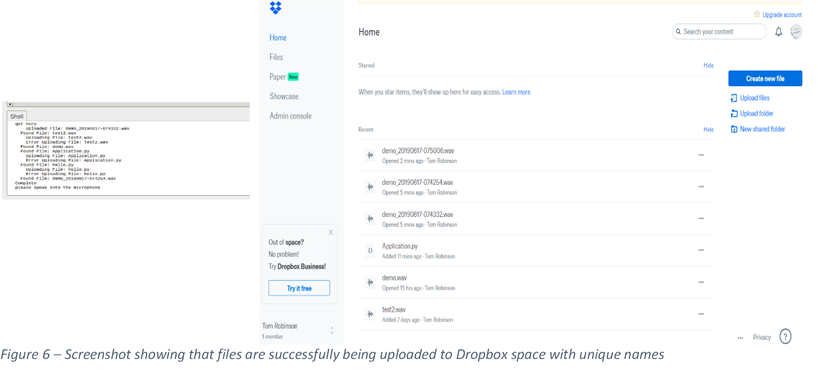
\includegraphics{Screenshot1.PNG}

These screenshots are showing these three are successful as there are files being uploaded to the system that are all named differently. You can see from the image on the left that the output of the console is telling you if the file has been uploaded successfully. You can also see from this image that a file already on the system will receive an error during the uploading process, also if this process was unsuccessful there would be no files viewable or repeat files with the same name on viewable on the Dropbox space. The screenshot below is showing that the file is also saving locally.\\

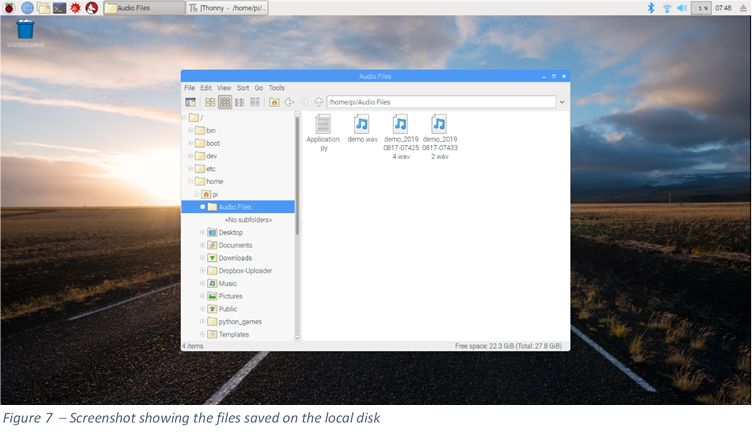
\includegraphics{Screenshot2.PNG}

The next image is showing that the system will activate on shouting being heard. It is also showcasing some of the reasons I decided to use Dropbox as the place to upload my files to, as it is showing the breakdown of the file into decibel level and is showing that comments can be added to the file.\\

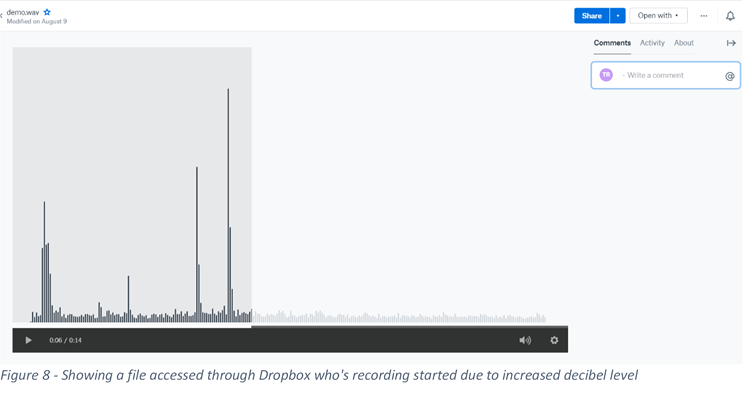
\includegraphics{Screenshot3.PNG}

Here you can see the loud noise that has been detected right at the start of the recording, indicating this was what activated the system. This screenshot is also showing that the recording will continue if there is another loud noise heard, if the system was to stop recording 5 seconds after the initial sound was heard the recording would be around 5-6 seconds long. But as you can see from the image that the final audible noise has occurred at 6 seconds, which has prolonged the recording to a total of 14 seconds, due to the addition of the silence I added in the processing. On the right hand side of the image there is the space to leave comments. \\

This image is showing that the conversation heard before the shouting will be recorded, up to 5 seconds long. As mentioned before, this number is changeable but for the purposes of demonstration it is set at this length.\\
\begin{center}
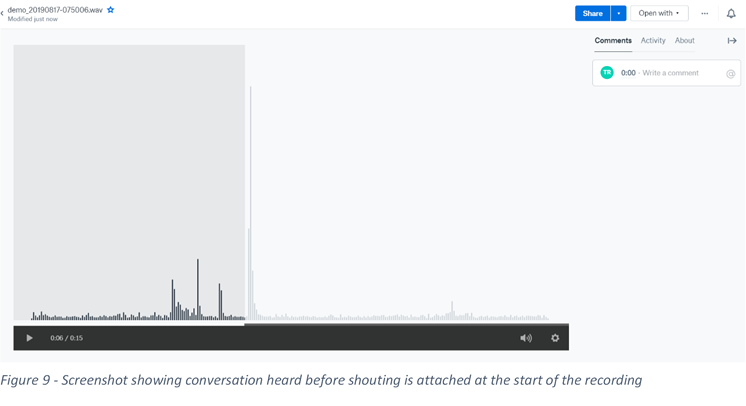
\includegraphics{Screenshot4.PNG}
\end{center}

This is showing the conversation heard before the shouting is recorded as the decibel level in the first 5 seconds does not reach above a level needed to constitute shouting but is still included in the recording, as you can see from this image that the talking heard does not exceed 5 seconds, when this reached 5 seconds you can see the application does not send the data and restarts the console. \\

\section{Evaluation}
Looking at the requirements I have set out at the start of this section I know the artefact has achieved all the aims to a certain degree. The first and second requirements were to gather useful information and to correctly identify a type of conversation, having outlined in the literature review that shouting is a sign of conflict, this has been fulfilled by having the system activate when shouting it occurring. Also adding to the first requirement is the recording of antecedent audio, giving context to the ensuing recording. I have established a clear-cut point in conversation that identifies when a conflict \textit{may} be occurring which \textit{should} be surrounded in useful information for analysis, which is what requirement 3 is asking for. Having exported the application into a Raspberry Pi I have given every chance for the project to be placed in range of ‘good’ conversations, which is what requirement 4 wants. This is because the Pi will only need to be connected to a power outlet which are usually placed in vocal points of a household. Requirement 5 is slightly achieved by exporting to Pi and having the used a case on top of it, the device is now just a small black box, which is nearly as inconspicuous as you can get. It doesn’t make any noise or create any lights so it should be accepted into the home with ease. Having copied the files into a place where the participants can access their recordings, I am considering data protection laws while still, hopefully, achieving a good amount of data to be analysed.\\

There are some areas in which this device does not achieve these aims as there is always a possibility that the device, which currently only has a small and relatively cheap microphone, may not detect the shouting. This is especially the case if the device is not placed in the room that the conversation is happening. As mentioned above, the project should be able to identify when a conflict is occurring, although there is a potential for certain conflicts to be missed due to this project only listening for a certain decibel level being reached. There may be cases in which the system detects shouting which is not related to an argument (e.g. trying to talk to someone in another room), but these will easily identifiable when they are opened for analysis.. As for requirement 5, regarding the device being accepted in the home, it will be difficult to judge how effectively the device has achieved this goal as the only the family will know the true dynamic of the house and it will be hard to tell if the device being in the home is in the sub-conscious of the participants. The fact that the data is being uploaded to Dropbox may impact this as the participants can easily see the amount of data being uploaded and they may be trying to keep this down if they are regularly checking. 

\chapter{DPICS \& SSP}
In this section I will be making comparisons between, and mapping, some of the techniques outlined in the \textit{Dyadic Parent-Child Interaction Coding System} (DPICS) to the methods currently available through \textit{Social Signal Processing} (SSP). These are purely potential projects that I have not attempted to complete, but from the research I have conducted, there is no comparisons between this emerging technology and the tried and tested manual. Below I am describing some SSP projects that could be used / adapted to aid in the automatic detection of the parental techniques outlined in DPICS.\\

One of the techniques outlined in DPICS is the difference between a \textit{Direct} and \textit{Indirect command} given by the parent to a child. It is also outlined in this manual that a direct command usually starts with the imperative verb and is often followed by a “Please”, “Thank you” or the child’s name. If this technique was hoping to be detected by a system it would be useful have to read the chapter informing readers about current state of the art methods for speech synthesis from ‘\textit{Social Signal Processing}’ (Georgila, 2017). Although this chapter’s main focus is the reproduction of speech it also outlines how to best convert the spoken word into something a computer can analyse. \\

This can be done in various ways which have been highlighted by Georgila, one area that could be of interest to this subject area is Emotional Speech Synthesis (aiming to capture and reproduce emotional speech). As this project is aimed at detecting the emotion rather than reproducing it, I am only interested in the early processes of capturing the emotional speech and the categorizing of data (used in the Hidden Markov Model method). After this has been done the specific words outlined above can be programmed into activating a system when heard, which could be done in a similar sense as to what my system is trying to achieve. Although those three words (“please”, “thank you” and the child’s name) are commonplace in a home there is a possibility to encode verbs, so should a verb be detected with these placed in the surrounding audio, the interaction can be classed as a direct command. DPICS also defines a direct command as being a positive command. Here SSP can also be used to observe various \textit{non-linguistic vocalizations} which can provide evidence for emotional states and social bonds.\\

Another behaviour that could be detected by SSP methods is that of Parent Ignore. This is defined as when “Deviant behaviour is ignored when parent remains silent, remains neutral, avoids or breaks eye contact with child, must last a minimum of 5 seconds” (Eyberg, 2000). This parental technique incorporates other techniques under \textit{deviant behaviours}, which covers some child behaviours: Cry, Whine, Yell, Smart Talk, Destructiveness and Physical Negative- Child. All of these can be a trigger / anchor point for this one to begin. Cry, Whine, Yell and Destructiveness could all possibly be detected using a decibel monitor, which would then activate a system on reaching a certain level and then record the ensuing data (either audio or video). Smart talk would make use of the similar techniques mentioned for \textit{Direct Commands} as it would analyse the emotional states by analysing the \textit{non-linguistic vocalizations}. Some work has been proposed that during a disagreement or a conflict there will be more engagement from parties in the room (Britta \& Elizabeth, 2003). For example, if there was to be a physical attack on someone, one would assume that there would be an increase in the amount activity detected as people come into the room to check on the victim. This could easily be achieved even through just listening for amount of different voices, tone of voice and by taking an average for interactions, e.g. duration models (distribution of speaking time across speakers), and lexical measurements (distribution of number of words over the utterance).\\

After the device has detected the deviant behaviour, the next step would then be how to decide if a parent has ignored the behaviour. There has been some work done on how one would detect the shape and posture of a subject, with much work being done on introducing a framework that aims to represent the shape of an activity by mapping the spatiotemporal localisation of certain features (Oikonomopoulos, Patras, \& Pantic, 2010). This work should be able to decide if the parent has changed body shape after the deviant behaviour has occurred, which would be useful in deciding if the parent has turned their back on the child / remained neutral. One disadvantage of using this method is that it is not able to define smaller movements, for example avoiding or breaking eye contact. This means that it would be able to automatically flag this behaviour as ‘Parent Ignore’.\\

One final behaviour from DPICS that could be detected using SSP technology is ‘Question’. This is defined in the DPICS manual as “... a comment expressed in question form”. There are a few different types of questions and a few ways of expressing a question in conversations which can make this a difficult category to accurately encode. One way DPICS encodes questions, which could be useful when trying to find an SSP method that is appropriate for detecting a question, is that the voice will rise rather than fall at the end of the sentence. Detecting a change in pitch has been used in a variety of ways in SSP so the technology is there. One example is ‘Agreement Detection in Multiparty Conversation’ (Germesin \& Wilson, 2009) which attempts to identify agreements using different features of speech, including prosody (pitch and speed rate). This project is said to have an accuracy of 45\% in successfully labelling groups of utterances an agreement or a disagreement. In another example pitch has again been used to help label agreements or disagreements, but this time the conversation is based in a business meeting (Hillard, Ostendorf, \& Elizabeth, 2003).\\

A specific type of question that is described in the DPICS manual is a rhetorical question. Rhetorical questions can fall under either the \textit{Question} or \textit{Reflective Question} category, DPICS separates the two instances depending upon whether the parents repeat the child’s words or not (reflective = repeat). This would be possible to encode with SSP as the capabilities to recognise words spoken is there so, if there was to be a flag for a question being asked (raised pitch) and there was a repeat of words spoken in the store of conversation the system would correctly identify a reflective question. To separate a \textit{question} from an \textit{acknowledgment}, one could compare the pitch levels at the end of an utterance or compare the content of the utterance, although this would require human input which is something this project is trying to reduce.

\chapter{Conclusion}
\section{Objective Achievement}
Looking back to my main aim mentioned at the start of section 3, my aim is to be able to create a device that can help in understanding and capture a participant’s home environment more effectively so that therapists, or such professionals, can obtain conversations that contain techniques that may be harmful to a child’s mental wellbeing. Overall, I think my device has achieved this in some ways, but there are also some improvements that could be made to the system to make the device even more effective in combating this problem. An important step of the process in making this a successful device was setting out the objectives for a device like this without considering the specific type of data I wanted to capture. This allowed me to be objective about what would make a good system for monitoring participants in their homes, while also being respectful to them and abiding by data protection laws should this software make it past the development stage.\\
 
I decided to make these aims more objective because of the research I performed before beginning the build for my project, in particular the DPICS manual. This manual, which covers a broad of range of parental techniques, is not restricted to just techniques that could be detected with a decibel monitor and audio recorder. Because of this I wanted to make my project as dynamic as possible, allowing it to be picked up again, by me or someone else, and that person to be able to build some functionality for a different technique in DPICS according to the broader objectives I have set out here. For the build, I feel I have been able to effectively reach a solution to the specific detection of shouting and capturing the surround audio with a relatively cheap solution, something that may be important in the wider distribution of the device should the device be taken further.\\

One thing outlined in the literature review was that it is important to focus new studies on the prevention of problems with mental health, rather than the treatment. This is where this study can hopefully be helpful as the focus is on the prevention of problems, aiming to detect early signs in the form of parental techniques. Even though the detection system may not be perfect I feel this is a step in the right direction, especially considering the ability of this device to be placed in the home, another thing that was outlined as being key in the collection of \textit{quality} data for studies of this manner. On top of the increased quality from the placement in the home I have been able to achieve a continuous stream of conversation which will enable the shouting to be analysed in context of what was happening in the home at the time, which was also found to be useful in the studies reported above. Something my report is adding to this area of research is the comparison of current abilities of SSP to the techniques in DPICS, which is something that had not been done before at time of writing. For the practical side of the project I am adding a study into the research of vocal behaviour in SSP, which was outlined as being an area that had limited studies prior to this project.  \\

Some issues with the system include the software not being implemented into devices already in the home, as outlined in the evaluation of the implementation, having a new device in the home in any capacity may affect the participants. It is also disappointing not to have the system implemented into an active voice assistant with this study being titled as it is, although the research surrounding the build are valid, regardless of the medium the audio is recorded from. Additionally, this software has not been tested on real life subjects, so I am unsure on how practically effective the system is. This is mainly due to time restrictions, specifically in getting the approval to record personal data of families and especially children. So sadly, the results gathered are only recordings that I have made by myself, which may be unintentionally biased. Also, my system is only built to detect one specific point in a conversation, which limits the types of conversations that can be recorded. 

\section{Future Work}
Despite the project achieving its main goals and, hopefully, adding some research into the study of vocal behaviour in detection of poor parental techniques, there are some ideas that could be implemented into this project that would increase its ability to help this area of study. The first thing that should be done to validate the results and findings in this report would be to test the system on actual families. This would allow the project to obtain useful results and from that point the software would be able to grow into something that is centred around the users experience with the system. Additionally, after obtaining results, these further improvements could be implemented to build on the detection of conversations of interest.\\

To make the system more capable of detecting when conflicts arise it would be useful to implement some of the other methods of detection that have been outlined in the DPICS \& SSP section above, which describes systems that use other sensors to decide whether there is a conflict taking place. It also outlines systems that detect whether the conversation taking place is an agreement or disagreement and ones that register emotional states. All three of these theories could be used on top of the detection of decibel level. The idea that a higher interaction rate would be registered in a room if a conflict was occurring is an interesting one that could be implemented into this system. However, to do this one would have to be able to identify the different parties that are involved in the conversation by analysing the prosody and lexical features of each talker. Having done this, one would be able to register the amount of people in the room, who was talking the most and with my system the volume in which these conversations were happening. Additionally, reading from the above literature, if that kind of detection was implemented, it would also be possible to detect if the participants in the specific conversations occurring in range of the sensor were starting to overlap each other and are ‘\textit{fighting}’ for the floor space, another sign that a conflict was taking place.\\

As I have made the project with a Raspberry Pi, there are other kinds of devices that can be attached that would give another dynamic to the project. One example would simply be a camera that would capture the video in view of the device as well as the audio. This would allow for the person analysing the situation to have a better understanding of who is part of the conversation and would be able to review more than just the audio features of the conversation. Opening this door would allow many more of the parental techniques from DPICS to be recorded, this would also squash any deniability for participants who were claiming not to be the offender in the situation. However, they would not be able to automatically detect any of the techniques with just a camera like the shouting currently is for my system. This could be done by adding a movement sensor, which could be used in a similar fashion to what has been described in section 4. But adding more sensors and data collectors to the device will make it less conspicuous, potentially effecting the quality of data collected.\\
  
An improvement that could increase the effectiveness of the system would be to make the project more interactable, which has been seen to yield some interesting and substantial data directly from the subjects, in a similar fashion to the study into schizophrenia or the study conducted with the child on an iPad (Can be found in the review of current techniques). Potentially including a brief survey for the subjects to complete once a day, in which they could be asked things like; how many times they think the device recorded conflicts, how intrusive they feel the device has been, how honest they think they have been around the device since its installation, etc. These results, used in conjunction with the data collected, will provide the therapist with participants views on themselves (which could be useful information in itself) and the experiment.\\

One final improvement I would make to the system is implementing a kind of sliding window in which the talking heard before the shouting moved in. In this system there would not be a set time for the recording of conversation, if the conversation time exceeds 5 seconds the system would remove the first second of talking heard and replace that space with an extra second of newer talking heard. This kind of system would allow for relevant data to be recorded as it means the talking immediately prior to the shouting is recorded but also ensures there is a complete flow of conversation in the saved file. This is an improvement on the current system as after 5 seconds of talking is heard the conversation is forgotten, for example, if the conversation leading up to the shouting was 7 seconds long the recording from my system would only be 2 seconds, which may not be enough time to give the context for the shouting. The improved system would always include 5 seconds of conversation as the sliding window would have removed the first 2 seconds, which is more likely to give a better account of the conversation.
\chapter{Appendix}
\section{Appendix 1 - Project Plan}

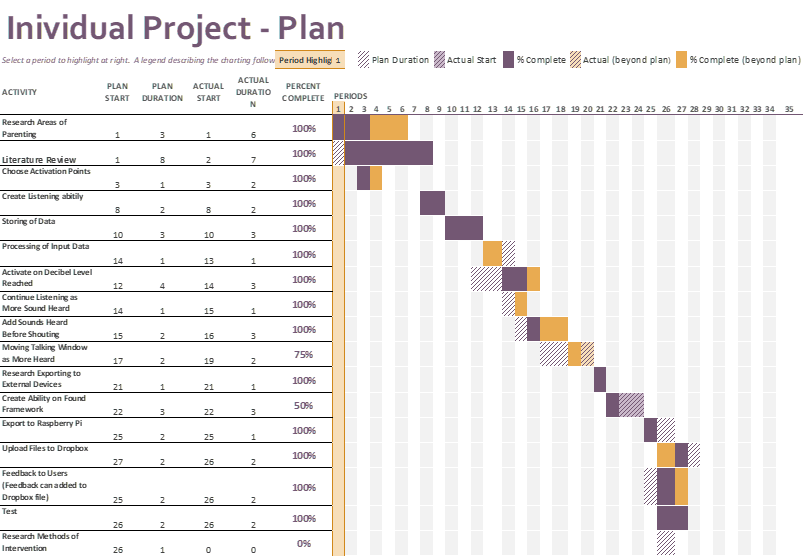
\includegraphics{Plan.PNG}
\pagebreak

\section{Appendix 2}
The further 9 points that they have outlined include:\\
\begin{itemize}
\item minimizing the gap between diagnosis and treatment
\item providing no shorter than three/four hours of treatment each day
\item involving the family
\item providing six-monthly development evaluations and updating the goals of treatment, 
\item choosing among behavioural/developmental treatment depending on the child’s response,
\item	encouraging spontaneous communication,
\item	promoting the skills through play with peers,
\item	gearing toward the acquisition of new skills and to their generalization and maintenance in natural contexts,
\item	supporting positive behaviours rather than tackling challenging behaviours. 
\end{itemize}

\chapter{References}
Amazon. (2017). \textit{Fitness Guru}. Retrieved from Amazon: https://www.amazon.com/Unisys-Fitness-Guru/dp/B0716PVZV4/ref=sr\_1\_1?s=digital-skills\&ie=UTF8\&qid=1497980936\&sr=1-1\&keywords=\\fitness\%20guru\&tag=cnet-vig-news-20\\

Amazon. (2017). \textit{My Workouts}. Retrieved from Amazon: https://www.amazon.com/Voice-Apps-LLC-My-Workouts/dp/B06XR9BL7M/ref=cm\_cr\_arp\_d\_product\_top?ie=UTF8\\

Andrews, G., \& Wilkinson, D. D. (2002). The prevention of mental disorders in young people. In M. J. Australia, \textit{Preventing Depression} (pp. 97-100). Medical Journal of Australia.\\

Aspland, H., \& Gardner, F. (2003). Observational Measures of Parent - Child Interaction: An Introductory Review. \textit{Child and Adolescent Mental Health Volume 8}, 136 - 143. doi:https://doi.org/10.1111/1475-3588.00061\\

Baker, N. (2019). \textit{SPY IN THE HOUSE}. Retrieved from The Sun: https://www.thesun.co.uk/tech/8837948\\/amazon-listening-alexa-echo-clips-record-woman-shower-sex-assault/\\

Britta, W., \& Elizabeth, S. (2003). Spotting "hot spots" in meetings: human judgments and prosodic cues. \textit{Interspeech}.\\

Charney, D., Reynolds, C. I., Lewis, L., \& al, e. (2003). Depression and Bipolar Support Alliance consensus statement on the unmet needs in diagnosis and treatment of mood disorders in late life. \textit{Arch Gen Phychiatry}, 664-672. doi:https://doi.org/10.1001/archpsyc.60.7.664\\

Cheng, D., \& Cristani, M. (2017). Social Signal Processing for Surveillance. \textit{Social Signal Processing}, 331-348.\\

Chetouani, M., Boucenna, S., Chaby, L., Plaza, M., \& Cohen, D. (2017). Social Signal Processing and Socially Assistive Robotics in Developmental Disorders. \textit{Social Signal Processing}, 398-403.\\

Dishion, T. J., Rivera, E. K., Jones, L., Verberkmoes, S., \& Patras, J. (2002). \textit{Relationship Process Code}. Unpublishedcoding manual. (Available from Child and Family Center,University of Oregon, 195 West 12th Avenue, Eugene, OR97401–3408, USA).\\

Eyberg, S. (2000, August). \textit{DYADIC PARENT-CHILD INTERACTION CODING SYSTEM: A MANUAL}. Retrieved from Incredible Years: http://www.incredibleyears.com/download/research/\\dpics-manual.pdf\\

Fabrizi, A. (2016, January). \textit{Dropbox Uploader}. Retrieved from Github: https://www.andreafabrizi.it/2016/01/01/Dropbox-Uploader/\\

Georgila, K. (2017). Speech Synthesis: State of the Art and Challenges for the Future. \textit{Social Signal Processing}, 257-272.\\

Germesin, S., \& Wilson, T. (2009). Agreement detection in multiparty conversation. \textit{Proceedings of the 2009 international conference on Multimodal interfaces}, (pp. 7-14).\\

Goleman, D. (2006). \textit{Social Intelligence}. Hutchinson.\\

Hillard, D., Ostendorf, M., \& Elizabeth, S. (2003). DETECTION OF AGREEMENT vs. DISAGREEMENT IN MEETINGS: TRAINING WITH UNLABELED DATA. \textit{Proceedings of the Conference of the North American Chapter of the Association for Computational Linguistics: Human Language Technologies}, (pp. 34-36).\\

Hiniker, A., Froehlich, J., Zhang, M., \& Beneteau, E. (2019). \textit{Anchored Audio Sampling}. New York: ACM.\\

Kääriä, A. (2017). \textit{Technology acceptance of voice assistants : anthropomorphism as factor}. Jyväskylä: University of Jyväskylä. Retrieved from http://urn.fi/URN:NBN:fi:jyu-201706202988\\

Lindsey (f4ngy). (2014). \textit{BarkTracker}. Retrieved from GitHub: https://github.com/f4ngy/BarkTracker\\

Mental Health Foundation. (2019). \textit{Children and Young People}. Retrieved from Mental Health Foundation: https://www.mentalhealth.org.uk/a-to-z/c/children-and-young-people\\

Mrazek, P., \& Haggerty, R. (1994). \textit{Reducing Risks for Mental Disorders: Frontiers for Preventive Intervention Research}. Washington DC: National Academy Press. Retrieved from https://books.google.co.uk/\\books?hl=en\&lr=\&id=5V66-WRcGL8C\&oi=fnd\&pg=PP30\&dq=Reducing+Risks+for+Mental+\\Disorders:+Frontiers+for+Preventive+Intervention+Research\&ots=N3amoaSes4\&sig=\\yYYHQgaNdl7OUoxvd8TprEOux2I\#v=onepagez\&q=Reducing\%20Risks\%20for\%20Mental\%20D\\

National Acadamies Press (US). (2009). \textit{Preventing Mental, Emotional, and Behaviour Disorders Among Young People}, Chapter 9. Retrieved from https://www.ncbi.nlm.nih.gov/books/NBK32775/\\

NHS . (2014). \textit{Adult Psychiatric Morbidity Survey: Survey of Mental Health and Wellbeing, England, 2014}. Retrieved from NHS England: https://webarchive.nationalarchives.gov.uk/20180328140249/\\http://digital.nhs.uk/catalogue/PUB21748\\

NHS. (2007). \textit{Adult Psychiatric Morbidity in England - 2007, Results of a household survey}. Retrieved from NHS Digital: https://digital.nhs.uk/data-and-information/publications/statistical/adult-psychiatric-morbidity-survey/adult-psychiatric-morbidity-in-england-2007-results-of-a-household-survey\\

NHS England. (2019). \textit{Mental Health Five Year Forward View Dashboard}. NHS England. Retrieved from https://www.england.nhs.uk/mental-health/taskforce/imp/mh-dashboard/\\

Oikonomopoulos, A., Patras, I., \& Pantic, M. (2010). Spatiotemporal Localization and Categorization of Human Actions in Unsegmented Image Sequences. \textit{IEEE Transactions on Image Processing}, 1126–1140.\\

Pargee. (2015). \textit{7-Minute Workout}. Retrieved from Amazon: https://www.amazon.com/Pargee-7-Minute-Workout/dp/B018WUNBE6/ref=sr\_1\_1?s=digital-skills\&ie=UTF8\&qid=1497981082\&sr=1-1\&\\keywords=7-minute\%20workout\&tag=cnet-vig-news-20\\

Porcheron, M., Fischer, J., Reeves, S., \& Sharples, S. (2018). Voice Interfaces in Everydat Life. \textit{Hun Factors in Computing Systems} (pp. 1-12). Montreal: ACM. doi:https://doi.org/10.1145/3173574.3174214\\

Schegloff, E. (2000). Overlapping talk and the organization of turn-taking for conversation. \textit{Language in Society}, 1-29.\\

Scherer, K., Schüller, B., \& Elkins, A. (2017). Computational Analysis of Vocal Expression of Affect: Trends and Challenges. \textit{Social Signal Processing}, 56-68.\\

Simo, B., Bamvita, J.-M., Caron, J., \& Fleury, M.-J. (2018). Predictors of mental health service use among individuals with high psychological distress and mental disorders. \textit{Psychiatry Research Volume 270}, 1122-1130. doi:https://doi.org/10.1016/j.psychres.2018.10.019\\

Skills For Care. (2018, June). \textit{Mental Health, Dementia and Learn Disabilities}. Retrieved from https://www.skillsforcare.org.uk/Document-library/Standards/Care-Certificate/Standard\%209\%20\%20CC\\\%20Workbook.pdf\\

SkyPaw Co. Ltd. (2017). \textit{Decibel X}. Retrieved from https://itunes.apple.com/us/app/decibel-x-db-dba-noise-meter/id448155923?mt=8\\

Trueman, C. (2015). \textit{Standard 9 Awareness of mental health, dementia and learning diability}. \\Academia.edu. Retrieved from https://www.academia.edu/36236506/Standard\_9\_Awareness\_of\_mental\\\_health\_dementia\_and\_learning\_disability\\

Vinciarelli, A. (2017). Socal Signal Processing for Conflict Analysis and Measurement. \textit{Socal Signal Processing}, 378-388.\\

Vinciarelli, A. (2017). Social Signal Processing for Automatic Role Recognition. \textit{Social Signal Processing}, 225-233.\\

Wang, R., Wang, W., Aung, M., Ben-Zeev, D., Brian, R., Campbell, A., . . . Walsh, M. (2017). Predicting Symptom Trajectories of Schizophrenia using Mobile Sensing. \textit{PACM Interact. Mob. Wearable Ubiquitous Technol. 1, 3}, 110-134. doi:https://doi.org/10.1145/3276145.3276157\\

World Health Organisiation. (2003). \textit{Investing in Mental Health}. Switzerland: World Health Organisation. Retrieved from https://apps.who.int/iris/bitstream/handle/10665/42823/9241562579.pdf\\

Zhang, A. (2016). {SpeechRecognition 3.8.1}. Retrieved from Python Software Foundation: \\https://github.com/Uberi/speech\_recognition\\

Zubrick, R. S., Silburn, R. S., Burton, P., \& Blair, E. (2000). Mental health disorders in children and young people: scope, cause and prevention. \textit{Australian and New Zealand Journal of Psychiatry}, 570-578. Retrieved from https://www.tandfonline.com/doi/full/10.1080/j.1440-1614.2000.00703.x?scroll=top\&need\\Access=true\\


\chapter{Hard Copy of Code}

import pyaudio\\
import wave\\
import os\\
import subprocess\\
import sys\\

from subprocess import Popen, PIPE\\
from sys import byteorder\\
from array import array\\
from struct import pack\\

shoutThresh = 1000          \# Decibel level needed to be reached for shouting\\
talkThresh = 50             \# Decibel level needed to be reached for talking\\
CHUNK\_SIZE = 700            \# Size of data chunks\\
FORMAT = pyaudio.paInt16\\    
device = 2                  \# Where microphone is attached\\
myChannel = 1               \# input channels (only 1)\\
RATE = 44100                \# Rate of recording\\

\# Location of directory which contains files to be uploaded\\
homeDirectory= os.getcwd()\\
\# Path to the Dropbox-uploaded shell script\\
uploadPath = homeDirectory + "/Dropbox-Uploader/dropbox\_uploader.sh"\\

restart = 1\\

\# Format for information from uploader to be output\\
def dropboxUploadOutput(msg, level):\\
    print((" " * level * 2) + msg)\\

\# What is Silent\\
def is\_silent (currentData):\\
    \#Returns 'True' if below the 'silent' talkThresh\\
    return max(currentData) < talkThresh\\

\# What is Shouting\\
def is\_shout (currentData):\\
    \#Returns 'True' if above shoutThresh\\
    return max(currentData) > shoutThresh\\

\# What is Talking\\
def is\_talk (currentData):\\
    \#Return 'True if between 'talkThresh' and 'shoutThresh\\
    return talkThresh < max(currentData) < shoutThresh\\

\# Bring recording into an average volume so it is at an acceptable level throughout\\
def averageVolume(currentData):    \\
    MAX = 15000\\
    \# Find aveage\\
    times = float(MAX)/max(abs(i) for i in currentData)\\
    r = array('h')\\
    \# Apply average to all data\\
    for i in currentData:\\
        r.append(int(i*times))\\
    return r\\

\# Remove blank data at the start and end of the recording\\
def concentrateData(currentData):\\
    def \_concentrateData(currentData):\\
        dataSending = False\\
        r = array('h')\\
        \#Find all data that is silent before the activation point\\
        for i in currentData:\\
            if not dataSending and abs(i)>talkThresh:\\
                dataSending = True\\
                r.append(i)             \\
                    

            elif dataSending:\\
                r.append(i)\\
                
        return r    \\

    \# Remove all appropriate data at start of recording\\
    currentData = \_concentrateData(currentData)    \\

    \# Remove all appropriate data at end of recording by;\\
    \# flipping all data, apply removal, flip back \\
    currentData.reverse()\\
    currentData = \_concentrateData(currentData)\\
    currentData.reverse()\\
    return currentData\\

\# After removing the potentially lengthy silences, add a short amount of silence \\
\# to both sides of recording so that the file feels more professional\\
def addSilence(currentData, seconds):\\
    r = array('h', [0 for i in range(int(seconds*RATE))])\\
    r.extend(currentData)\\
    r.extend([0 for i in range(int(seconds*RATE))])\\
    return r\\

\# Retrieves files in Dropbox directory in child program and returns them as a list to main program\\
def listDropboxFiles(path):\\
    \# Open child program\\
    p = Popen([uploadPath, "list", path], stdin=PIPE, stdout=PIPE, stderr=PIPE)\\
    \# Format output\\
    output = p.communicate()[0].decode("utf-8")\\

    outputList = list()\\
    lines = output.splitlines()\\

    \# Neaten output data into separate lines\\
    for line in lines:\\
        if line.startswith(" [F]"):\\
            line = line[5:]\\
            line = line[line.index(' ')+1:]\\
            outputList.append(line)\\
                   
    return outputList\\

\# This class gets the files from the local drive, compares to dropbox space, \\
\# plus uploads new file if no match\\
def uploadToDropbox(path, level):\\
    homePath = os.path.join(homeDirectory,path)\\
    dropboxUploadOutput("Syncing " + homePath,level)\\

    if not os.path.exists(homePath):\\
        dropboxUploadOutput("No path at: " + path, level)\\
    else:\\
        \# List files and directories in local space\\
        localSpace = os.listdir(homePath)\\

        \# Group      \\
        files = list()\\
        directories = list()\\

        \# For everything in the local space, add to either 'files' or 'directories'\\
        for file in localSpace:\\
            fileAddress = os.path.join(homePath,file)\\
            if os.path.isfile(fileAddress):\\
                files.append(file)       \\
            if os.path.isdir(fileAddress):\\
                directories.append(file)\\

        \# Let user know how many directories and files found\\
        dropboxUploadOutput(str(len(directories)) + " Directories, " + str(len(files)) + " Files ",level)\\

        \# Get list of files in dropbox\\
        if len(files) > 0:\\
            dropboxFiles = listDropboxFiles(path)\\

        \# For each file, check if the file can be uploaded properly\\
        for f in files:                                 \\
            dropboxUploadOutput("Found: " + f,level)   \\
            if not f in dropboxFiles:\\
                fullAddress = os.path.join(homePath,f)\\
                relativeAddress = os.path.join(path,f)  \\
                dropboxUploadOutput("Uploading: " + f,level+1)   \\
                if fileUpload(fullAddress, relativeAddress) == 1:\\
                    dropboxUploadOutput("Upload Complete for: " + f,level + 1)                                  \\          
                else:\\
                    dropboxUploadOutput("Error With File: " + f,level + 1)\\
                    
        \# Loop through directories within local space       \\
        for d in directories:\\
            dropboxUploadOutput("Directory: " + d + "found", level)\\
            directoryPath = os.path.join(path,d)\\
            uploadToDropbox(directoryPath, level + 1)\\

\# Process of uploading a single file \\
def fileUpload(localPath, remotePath):\\
    p = Popen([uploadPath, "upload", localPath, remotePath], stdin=PIPE, stdout=PIPE, stderr=PIPE)\\
    output = p.communicate()[0].decode("utf-8").strip()\\
    \# If the output starts and finishes with these two messages then the file will have been uploaded\\
    \# successfully through 'Dropbox\_Uploader' program\\
    if output.startswith("> Uploading") and output.endswith("DONE"):\\
        print ("got here")\\
        return 1\\
    else:\\
        return 0\\

\# Class that handles the setting up of audio stream, activating system on decibel level reached, \\
\# appropriate collection of data surrounding anchor point, restarts system if no shouting detected \\
\# and applies processing\\
def record():       \\
    shoutingLoop = 1\\
    \# While the system hasn't heard shouting\\
    while shoutingLoop == 1 :\\
        \# Open stream\\
        p = pyaudio.PyAudio()\\
        stream = p.open(format=FORMAT, channels=myChannel, rate=RATE, input\_device\_index = device,\\
            input = True, output = True,\\
            frames\_per\_buffer=CHUNK\_SIZE)\\

        \# Counters\\
        num\_silent = 0\\
        talkTime = 0\\
    
        dataSending = False\\
        shoutingNotDetected = True\\
        talkDetected = False\\
        recordingLoop = 1    \\

        r = array('h')\\

        \# While neither counter has reached its capacity and system needs to listen for new data\\
        while recordingLoop < 2 :\\
            \# Associate new data chunks with current data object\\
            currentData = array('h', stream.read(CHUNK\_SIZE))\\

            if byteorder == 'big':\\
                currentData.byteswap()\\
            r.extend(currentData)\\

            silent = is\_silent(currentData)\\
            talk = is\_talk (currentData)\\
            shout = is\_shout(currentData)               \\
        
            \# While shoutingNotDetected:\\
            \# If talking heard set to true            \\
            if talk:\\
                talkDetected = True\\

            \# If time since talking is below 5 seconds, keep sending data\\
            if talkTime < 500:\\
                dataSending = True\\

            \# If time since talking initially heard exceeds 5 seconds, reset timer and tell user no shouting heard\\
            if talkTime >= 500:\\
                print ("No shouting heard in last 5 seconds, reset memory")                \\
                talkTime = 0                         \\
                print ("Not sending data")\\
                \# Break recording loop, so that a new stream can be opened, deleting old data (with no shouting)\\
                recordingLoop = 3 \#BREAK\\

            if talkDetected == True:                \\
                talkTime += 1\\
                \#print (talkTime)\\
             
            \# When shouting is detected, set boolean to true \& reset talking timer\\
            if shout:\\
                print ("Shouting Detected")\\
                shoutingNotDetected = False\\
                \#dataSending = True            \\
                talkTime = 0\\

            \#Increase silence time if send has started and nothing is heard\\
            if silent and dataSending == True:\\
                num\_silent += 1\\

            \# If there is silence and shouting has been detected, the talking timer will be set to 0\\
            \# (so talk time doesn't reach maximum and stop recording)\\
            if silent and not shoutingNotDetected:\\
                print ("Waiting ...")\\
                talkTime = 0\\
                \#print (num\_silent)   \\

            \#Reset silence timer if any audio is heard as to extend the recording\\
            if not silent and dataSending == True:\\
                print ("Reset Timer, More Heard") \\
                num\_silent = 0\\

            \# If sending has started, shouting is hear and the number of silence is greater than 5 seconds\\
            if dataSending == True and not shoutingNotDetected and num\_silent > 500:\\
                \# Break the recording loop\\
                recordingLoop == 4 \#BREAK\\
                break    \\
        
        \# Get size of file in chunks + stop and close audio stream\\
        sample\_width = p.get\_sample\_size(FORMAT)\\
        stream.stop\_stream()\\
        stream.close()\\
        p.terminate()\\
        
        \# Check if shouting has been heard before applying the processing and saving of file\\
        if not shoutingNotDetected:\\
            shoutingLoop = 2 \#BREAK\\

    \# Process data according to classes\\
    r = averageVolume(r)\\
    r = concentrateData(r)    \\
    r = addSilence(r, 0.5)\\
    return sample\_width, r\\

\# Records data from the microphone selected and saves it to the local disk \\
\# with same properties as data from record class above \\
def convertToFile(path):\\
    sample\_width, data = record()\\
    data = pack('<' + ('h'*len(data)), *data)\\

    wf = wave.open(path, 'wb')\\
    wf.setnchannels(1)\\
    wf.setsampwidth(sample\_width)\\
    wf.setframerate(RATE)\\
    wf.writeframes(data)\\
    wf.close()\\

\# Path the program will take on start up\\
if \_\_name\_\_ == '\_\_main\_\_':   \\
    \# Infinite loop so system will always records if active \\
    while restart == 1:\\
        print("please speak into the microphone")\\

        \# First file to be named 'demo.wav' as this should be a test of the system \\
        \# Rest of files to be named with date and time\\
        if os.path.exists('demo.wav'):\\
            import time\\
            timestr = time.strftime("\%Y\%m\%d-\%H\%M\%S")\\
            convertToFile('demo\_\{\}.wav'.format(timestr))\\
            print("Done - result saved 1")\\
        else:\\
            convertToFile('demo.wav')\\
            print("Done - result saved 2")\\

        \# After saving file locally, upload to dropbox\\
        uploadToDropbox("",1)\\

        print("Complete")\\

        \# Restart\\
        restart = 1\\


\end{document}